\chapter{Conceptual Design}
\label{chap:05_design}

In this chapter, the conceptual design of the implementation is introduced. This chapter's concept is based on the theory of \Chap{chap:02_foundation} and uses the technologies introduced in \Chap{chap:04_background}.


% ===========================================
% ===========================================
\section{Choice of Technologies}
\label{sec:05_restrictions}
The following technologies are used to create the conceptual design of the implementation:

\begin{itemize}
% python
\item Python programming language: Python is used as the main programming language for Apache Spark applications.

% docker
\item Docker: Docker is used to deploying components in the computing environment as a container. This enables to create homogeneous nodes in the environment. Furthermore, Docker Swarm is used as an orchestration tool and takes care of each component's health status.

% Gitlab
\item GitLab: The source code repository is hosted on the GitLab platform. Furthermore, the automated deployment pipeline is designed using the CI/CD feature of GitLab. Therefore, using GitLab fulfils the version control and build server requirements mentioned in \Sec{sec:02_depl-pipeline_requirements}.

% Spark
\item Apache Spark: Apache Spark is used to distribute the workload of training machine learning applications across multiple workers. The goal is to scale the replicas of Apache Spark workers to increase the performance of the cluster.

% RAPIDS
\item NVIDIA RAPIDS: In addition to scaling Apache Spark worker node replicas, the NVIDIA RAPIDS plugin suite is used to enable \hyperlink{abbr:gpu}{GPU} acceleration on the Apache Spark cluster. Enabling Apache Spark to leverage \hyperlink{abbr:gpu}{GPUs} increases the computational power as well.

% Prom
\item Prometheus: 
Prometheus fulfils all requirements of a monitoring system introduced in \Sec{sec:02_monitoring}. It provides a powerful multi-dimensional data-model and a query language for aggregations and filtering of multi-dimensional time-series data. Additionally, Prometheus is a pull-based monitoring system and includes a time-series database.

% cAdvisor
\item cAdvisor:
cAdvisor serves as a monitoring agent. It scrapes performance metrics from Docker containers. Prometheus pulls the data from cAdvisor to save it in its time-series database.

% dcgm-exporter
\item DCGM-Exporter:
The DCGM-Exporter is used as a monitoring agent as well. It is used to monitor the utilization of the available \hyperlink{abbr:gpu}{GPUs}.
\end{itemize}


% ===========================================
% ===========================================
\section{Computing Environment Architecture}
\label{sec:05_env}
% Single machine
The computing environment is deployed on a single machine.
% Autonomic
The goal is to create a self-optimizing autonomic computing environment (described in \Sec{sec:02_ac}).
% manage
Furthermore, to manage the environment's components and resources, an autonomic manager is designed according to the \hyperlink{abbr:mape}{MAPE} architecture (introduced in \Sec{subsec:02_ac_manager}).
% Docker
For simplicity, each node in the computing environment is deployed as a Docker service in a Docker swarm (introduced in \Sec{subsec:04_docker_swarm}).
% swarm
This allows to define the state of each service, which includes the number of replicas. The number of replicas can be updated during runtime.


% Overall design
\begin{figure}[h]
\centering
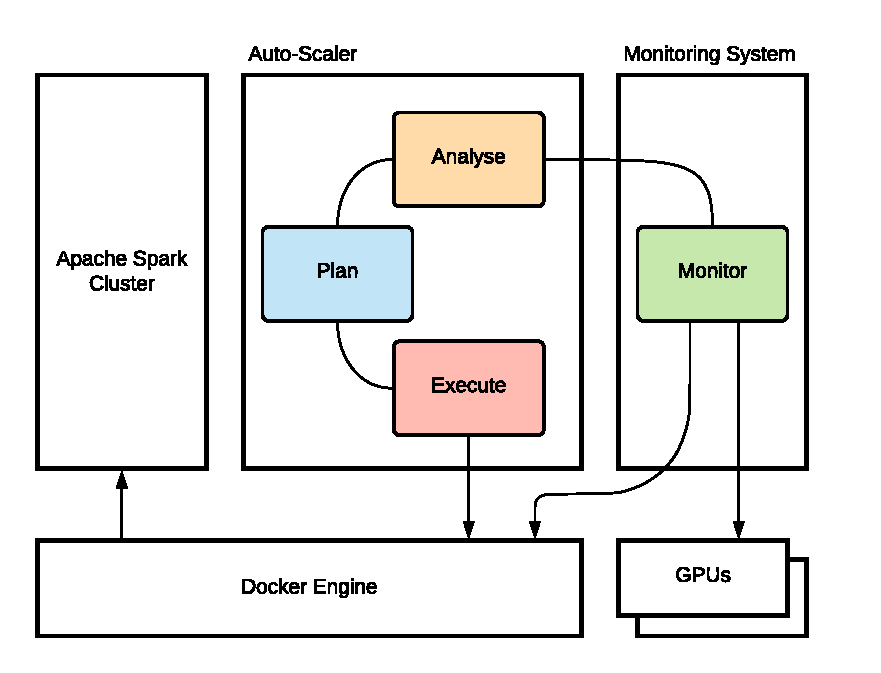
\includegraphics[scale=1]{images/05_conceptual_design/autonomic_manager/control_loop}
\caption{Full MAPE control loop architecture}
\label{fig:05_am_monitoring_loop_arch}
\end{figure}
% Explain 
\Fig{fig:05_am_monitoring_loop_arch} provides an overview of the computing environment concept.
% resources
The managed resources (introduced in \Sec{subsec:02_ac_resources}) in this environment are the Apache Spark cluster and the \hyperlink{abbr:gpu}{GPUs}.
% manager
These resources are managed by the autonomic manager, which consists of the \textit{Auto-Scaler}, and the monitoring system. Furthermore, the autonomic manager implements all four phases of the \hyperlink{abbr:mape}{MAPE} architecture and executes the control-loop.
% Docker 
As mentioned previously, all components are deployed using Docker. Therefore, to manage components in the computing environment, the autonomic manager needs to interact with the overlaying Docker engine.


\paragraph{Control-loop workflow:}
% Workflow figure
\begin{figure}[h]
\centering
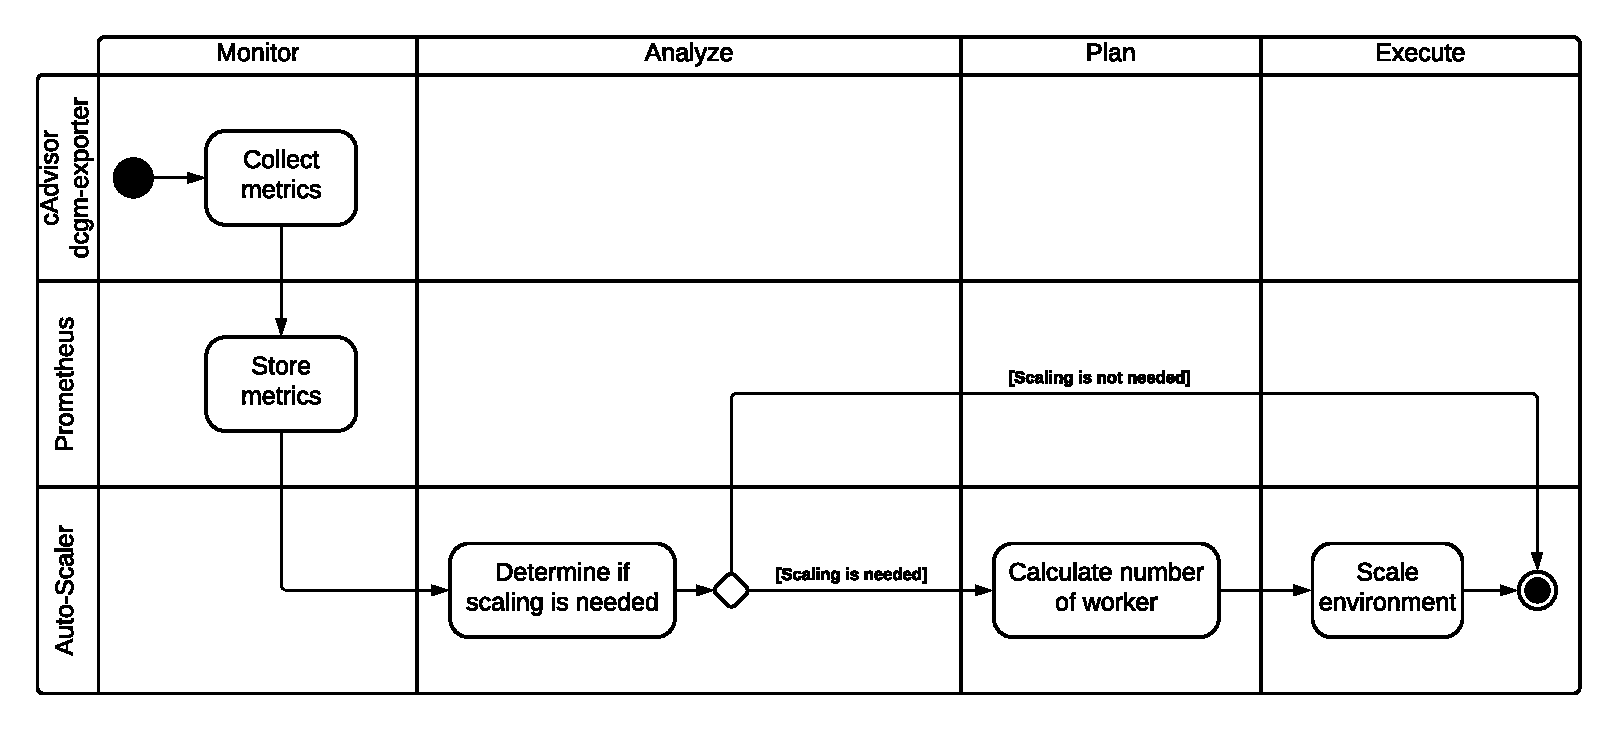
\includegraphics[scale=0.50]{images/05_conceptual_design/autonomic_manager/autonomic_manager_workflow}
\caption{UML activity model of the autonomic manager process}
\label{fig:05_am_monitoring_loop_workflow}
\end{figure}
% Explain
The control-loop workflow is illustrated in \Fig{fig:05_am_monitoring_loop_workflow}.
% Monitor
It starts in the Monitor phase. All monitoring agents (cAdvisor and DCGM-Exporter) collect performance metrics from their targets. Next, Prometheus pulls the metrics from all monitoring agents and saves the data in its time-series database.
% Analyze
In the analyse phase, the \textit{Auto-Scaler} determines if a scaling action is necessary. If a scaling action is not needed, the iteration ends.
% Plan
Otherwise, the \textit{Auto-Scaler} determines the number of Apache Spark worker replicas in the Plan phase.
% Execute
Lastly, in the Execute phase, the \textit{Auto-Scaler} scales the Apache Spark worker Docker service's replicas.


% ===========================================
% ===========================================
\section{Apache Spark Cluster}
\label{sec:05_spark}
% Short intro
The Apache Spark cluster is the computing unit of the environment. It is responsible for distributing the workload of training machine learning models.

\begin{itemize}
% Master
\item Master: The master is responsible for distributing the workload of an application, submitted by a \textit{spark-submit} node, across all available worker nodes. The Apache Spark application architecture is explained in \Sec{subsec:04_spark_architecture}.

% Worker
\item Worker: A worker node is responsible for performing the workload given by the master node. Furthermore, the replicas of active worker nodes in the cluster are dynamically adapted by the \textit{Auto-Scaler} at runtime.

\item Spark-Submit: A \textit{spark-submit} node is deployed whenever an application is submitted to the cluster.
\end{itemize}
% Figure
\begin{figure}[h]
\centering
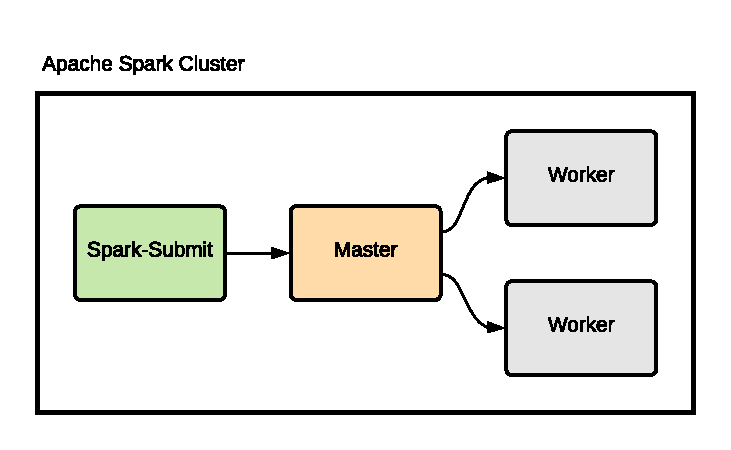
\includegraphics[scale=1]{images/05_conceptual_design/apache_spark/apache_spark_cluster}
\caption{Apache Spark cluster architecture}
\label{fig:05_spark_arch}
\end{figure}
% FIgure intro
\Fig{fig:05_spark_arch} illustrates the architecture of the Apache Spark cluster. It consists of a master node, multiple worker nodes, and spark-submit nodes.
% Standalone mode
The cluster is deployed in standalone mode (\Sec{subsec:04_spark_standalone}). Because Docker Swarm is used as the orchestration tool that controls nodes' state, there is no need to use another orchestration tool like Apache Mesos or Kubernetes as the cluster manager.
% Docker
Additionally, this simple approach allows running each node of the cluster in a Docker container without additional configuration.


\subsection{Homogeneous Apache Spark Worker Nodes}
% Short intro
The \textit{Auto-Scaler} scales the replicas of Apache Spark worker nodes. Therefore, the cluster is scaled horizontally. As explained in \Sec{subsec:02_foundations_scalability_horizontal-scaling}, the horizontal scaling approach is more efficient when scaling homogeneous nodes Each node adds the same amount of computational power to the cluster.
% How to achieve
To ensure that the worker nodes are homogeneous, the worker service uses the same Docker image for each worker node. The Docker image is created from a custom Dockerfile.
% Resources
This guarantees that each worker uses the same software and has the same amount of computational resources available.
% RAPIDS
Additionally, all requirements mentioned in \Sec{subsec:04_rapids_req} to enable \hyperlink{abbr:gpu}{GPU} acceleration with RAPIDS are installed in a worker image.


\subsection{Deploying an Application with spark-submit}
\label{subsec:05_spark_spark-submit}
% Intro
Whenever the \hyperlink{abbr:ci}{CI} pipeline submits an application to the Apache Spark cluster, it deploys a \textit{spark-submit} Docker container.
% spark-submit purpose
The \textit{spark-submit} container's purpose is to submit an application with the spark-submit executable (described in \Sec{subsubsec:04_spark_standalone_submit}) to the cluster.
% Resources
Additionally, the \textit{spark-submit} container sets the number of resources for the executors running on the worker nodes.
% No support for python in cluster mode
Apache Spark cluster's standalone mode does not support submitting Python applications with the spark-submit executable from outside of the cluster. Therefore, the spark-submit executable must be executed on the host machine with access to the master node \cite{Apache2020Spark}.
% Swarm
To submit an application to the master node, the \textit{spark-submit} container needs to be in the same Docker swarm network. The node is deployed as a Docker container instead of a Docker service. Each spark-submit container is deployed with a different setting depending on the configuration and application of the \hyperlink{abbr:ci}{CI} pipeline.
% End
After the application has been submitted, the spark-submit node automatically exits.


\section{Autonomic Manager}
\label{05_am}
% SHort intro
The autonomic manager is one of the main modules of the computing environment.
% Responsibilites
It is responsible for monitoring all Apache Spark worker node performance metrics and automatically scales the number of worker nodes to adapt to a specified performance goal.
% MAPE
The autonomic manager is implemented according to the \hyperlink{abbr:mape}{MAPE} architecture, as described in \Sec{subsec:02_ac_manager}. To create a complete control-loop, the autonomic manager comprises multiple components, as illustrated in \Fig{fig:05_am_concept}.
% A figure explaining the concept
\label{subsec:05_am}
\begin{figure}[h]
\centering
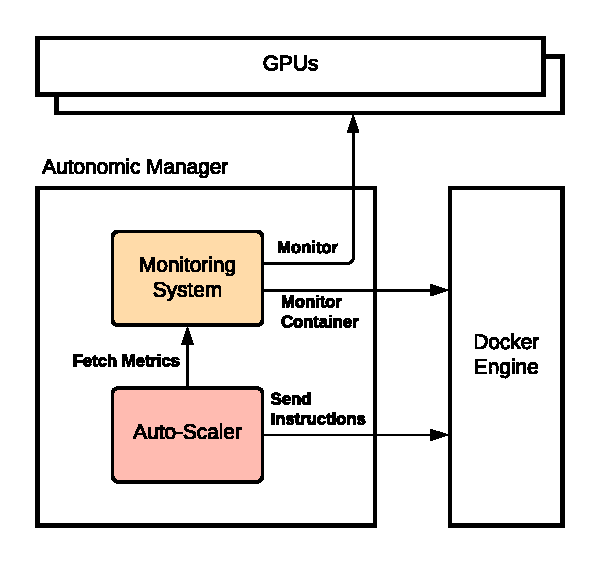
\includegraphics[scale=1]{images/05_conceptual_design/autonomic_manager/autonomic_manager_concept}
\caption{Autonomic manager component design}
\label{fig:05_am_concept}
\end{figure}
% Explain figure
It consists of a monitoring system (see \Sec{sec:02_monitoring}) and an \textit{Auto-Scaler} module.
% Docker
Each component in the computing environment is deployed as a Docker service. Therefore, Docker swarm takes care of the health status of each component.
% Monitor
To monitor overall Docker container performance in the computing environment, the autonomic manager needs access to the overlaying Docker engine. Additionally, to monitor \hyperlink{abbr:gpu}{GPU} performance, a monitoring agent is needed to scrape metrics from the \hyperlink{abbr:gpu}{GPUs}.
% Scaling
Furthermore, the autonomic manager is responsible for scaling the replicas of Apache Spark worker nodes. As introduced in \Sec{sec:05_spark}, a worker service takes care of all worker nodes. Therefore, the autonomic manager needs access to the host machine's Docker Engine in order to send scaling instructions.


\subsection{Monitoring System}
% Short intro
The monitoring system is responsible for performing the Monitor phase. Therefore it monitors the performance of components in the computing environment and makes them available to the \textit{Auto-Scaler}.
% Responsibilites
In this environment, the monitoring system collects worker container performance metrics, and the \hyperlink{abbr:gpu}{GPU} performance. It is essential to mention that the number of worker nodes varies over time because the \textit{Auto-Scaler} scales the worker nodes' replicas according to the system performance.
% The figure
\begin{figure}[h]
\centering
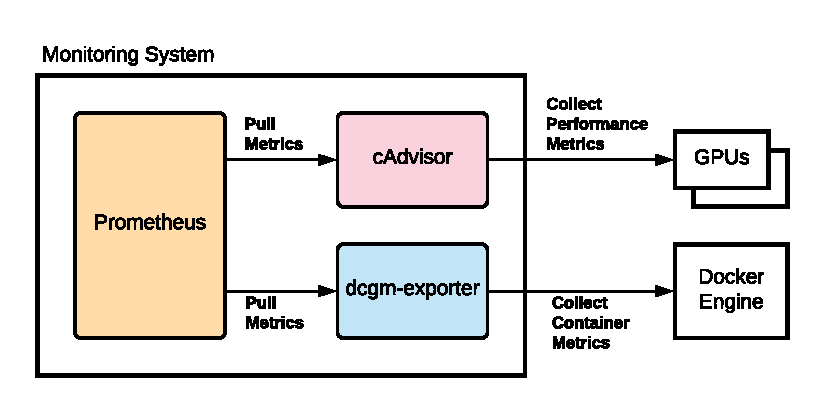
\includegraphics[scale=1]{images/05_conceptual_design/autonomic_manager/monitoring_system_concept}
\caption{Monitoring system conceptual design}
\label{fig:05_am_monitoring_concept}
\end{figure}
% Explain figure
\Fig{fig:05_am_monitoring_concept} illustrates the architecture of the monitoring system, which consists of three components:
% The components
\begin{itemize}
\item DCGM-Exporter: A monitoring agent that is responsible for collecting \hyperlink{abbr:gpu}{GPU} performance metrics.

\item cAdvisor: A monitoring agent that collects performance metrics of Docker containers in the environment.

\item Prometheus: It collects the performance metrics from all monitoring agents and saves them as time-series data in a time-series database.
\end{itemize}


\subsection{Auto-Scaler}
% Short intro
The \textit{Auto-Scaler} is the second module of the autonomic manager and responsible to dynamically adjust the replicas of Apache Spark worker nodes in the computing environment to accommodate specified performance goals. 
% MAPE
It implements the Analyse, Plan, and Execute phases of the \hyperlink{abbr:mape}{MAPE} architecture. Together with the monitoring system, it creates a complete autonomic manager implementing all phases of the \hyperlink{abbr:mape}{MAPE} architecture.
% Reactive threshold based 
The \textit{Auto-Scaler} is designed as a reactive auto-scaler and uses a threshold-based algorithm to scale worker nodes. To define the thresholds, it can be configured using a configuration file.


% Prom API
As illustrated in \Fig{fig:05_am_concept}, the \textit{Auto-Scaler} fetches performance metrics from the Prometheus \hyperlink{abbr:http}{HTTP} \hyperlink{abbr:api}{API}.
% Phases
After it received the performance metrics, the \textit{Auto-Scaler} analyses the metrics, plans scaling-actions to adjust the number of worker replicas, and sends instructions to the Docker engine.


\subsubsection{MAPE Phases}
% SHort intro
Mentioned above, the \textit{Auto-Scaler} implements the Analyse, Plan, and Execute phases of the \hyperlink{abbr:mape}{MAPE} architecture. Each phase has a different workflow to accommodate its goal.

\paragraph{Analyse:}
% How to analyze
During each period, the \textit{Auto-Scaler} fetches the performance metrics defined in the configuration file from the Prometheus \hyperlink{abbr:http}{HTTP} \hyperlink{abbr:api}{API}.
% Determine if scaling is needed
After the metrics are received, the \textit{Auto-Scaler} determines if a scaling action is needed using the Scaling Heat algorithm (introduced in \Sec{sec:04_background_scaling-heat}). If scaling is not necessary, the \textit{Auto-Scaler} continues to collect and analyse performance metrics.

\paragraph{Plan:}
% Short intro
If a scaling action is necessary, the \textit{Auto-Scaler} is responsible for determining the number of Apache Spark worker replicas needed to reach the defined utilization goal.
% Calculating Spark worker
To calculate the number of worker nodes, the \textit{Auto-Scaler} uses the Kubernetes Horizontal Pod Auto-Scaling algorithm (introduced in \Sec{sec:04_background_khpa}).
% Thresholds
If number of needed replicas violates the upper or lower thresholds of active Apache Spark worker nodes, the \textit{Auto-Scaler} uses the maximum or the minimum number of worker nodes as the desired replicas.

\paragraph{Execute:}
% Short intro
After the number of needed replicas have been calculated, the \textit{Auto-Scaler} sends the instruction to scale the Apache Spark worker service to the desired number of replicas.
% Cooldown
Afterward, a cooldown period is activated, which has the effect that the Apache Spark cluster needs time to distribute the workload across all new worker nodes efficiently. During the cooldown period, no scaling actions are executed.


\subsubsection{Configuration}
\label{subsubsec:05_am_auto-scaler_config}
The \textit{Auto-Scaler} needs specific configuration properties to collect the correct metrics from Prometheus and scale the Apache Spark worker service replicas. The following are properties that have to be defined to ensure that the \textit{Auto-Scaler} can collect meaningful metrics and scale Apache Spark workers as expected.

\begin{itemize}
\item General properties:
\begin{itemize}
\item Interval seconds: The number of seconds after the \textit{Auto-Scaler} starts a new process.

\item Cooldown period: The duration in seconds the \textit{Auto-Scaler} has to wait after a scaling action is performed.

\item Recurrence factor: To prevent too many scaling actions,  the autonomic manager should only execute a scaling action,  if the utilization thresholds are violated $n$ times.

\item Prometheus \hyperlink{abbr:url}{URL}: The Uniform Resource Locator (\hyperlink{abbr:url}{URL}) of the Prometheus \hyperlink{abbr:http}{HTTP} \hyperlink{abbr:api}{API}.
\end{itemize}

\item Metrics:
It is possible to define a list of metrics, where each metric needs to have a variety of properties configured.
\begin{itemize}
\item Target utilization: The desired utilization of the performance metric.

\item Utilization thresholds: To determine if a scaling action is needed, the scaling heat algorithm needs the minimum and maximum utilization of the performance metric.

\item Query: A PromQL query defines a performance metric.
\end{itemize}

\item Apache Spark worker properties:
\begin{itemize}
\item Worker service name: The Docker worker's service name is needed to update the number of replicas.

\item Worker thresholds: The maximum and the minimum number of concurrent Spark workers should be defined. To avoid the cold start effect, the minimum amount of workers should be at least 1. 

\item Apache Spark master \hyperlink{abbr:uri}{URI}: To distribute the Spark Worker workload, all Spark Worker need to communicate with the Spark master.
\end{itemize}
\end{itemize}


% ===========================================
% ===========================================
\section{Identification of Suitable Metrics for Scaling}
\label{sec:05_metrics}
% SHort intro
Suitable metrics are needed to measure the system performance while the Apache Spark cluster is actively performing work.
% Rapids enabled GPU
With the RAPIDS accelerator for Apache Spark, the cluster utilizes \hyperlink{abbr:cpu}{CPU} and \hyperlink{abbr:gpu}{GPU} computing power to enable parallelization.
% SO?
Therefore, suitable metrics to measure the system performance are the \hyperlink{abbr:cpu}{CPU} and \hyperlink{abbr:gpu}{GPU} utilization when the cluster is actively performing computations.


\subsection{CPU Utilization}
% Sharing CPU cores
All Apache Spark workers run on the same machine. Therefore, all available \hyperlink{abbr:cpu}{CPU} cores on the machine are shared across each Apache Spark worker.
%
To get a value that indicates the \hyperlink{abbr:cpu}{CPU} utilization between 0\% and 100\%, a metric is needed that represents the percentage of time all performing applications occupy \hyperlink{abbr:cpu}{CPU} cycles.
% cadvisor
cAdvisor provides a performance metric called \texttt{container\_cpu\_usage\_seconds\_total}\footnote{Monitoring cAdvisor with Prometheus - \url{https://github.com/google/cadvisor/blob/master/docs/storage/prometheus.md} (Accessed: 2021-01-21)}. This metric provides the total amount of \hyperlink{abbr:cpu}{CPU} seconds consumed by core of a container. 
% Overall utilization
To calculate the overall \hyperlink{abbr:cpu}{CPU} utilization for all Apache Spark worker, the value of the performance metric for each worker container over a specific rate is summed up.
%
In this case, the \hyperlink{abbr:cpu}{CPU} utilization ($U_{CPU}$) is defined by \Eq{eq:05_metrics_cpu} with $n \in \mathbb{N}$ the number of active workers.

\begin{equation}
U_{CPU}=\sum_{n=1}^{\mathbb{N}}container\_cpu\_usage\_seconds\_total_{n}
\label{eq:05_metrics_cpu}
\end{equation}

\subsection{GPU Utilization}
%
In addition to the \hyperlink{abbr:cpu}{CPU} utilization, Apache Spark workers can utilize \hyperlink{abbr:gpu}{GPUs} to accelerate the computation work.	
% The metric
The dcgm\_exporter agent provides the \texttt{dcgm\_fi\_dev\_gpu\_util} performance metric. This metric returns the percentual utilization per \hyperlink{abbr:gpu}{GPU}.
% How to calculate
Therefore, the \hyperlink{abbr:gpu}{GPU} utilization ($U_{GPU}$) is defined by \Eq{eq:05_metrics_gpu} with $n \in \mathbb{N}$ the number of available \hyperlink{abbr:gpu}{GPUs}.


\begin{equation}
U_{GPU} = \dfrac{\sum_{n=1}^{\mathbb{N}}dcgm\_fi\_dev\_gpu\_util_{n}}{\mathbb{N}}
\label{eq:05_metrics_gpu}
\end{equation}


% ===========================================
% ===========================================
\section{Automated Deployment Pipeline}
\label{sec:05_pipeline}
% Abstract
This thesis aims to train Machine Learning models by automatically submitting Apache Spark applications to an Apache Spark cluster. Therefore, the training process of a model has to be integrated into the application development lifecycle.
%
The application development lifecycle is automated using a deployment pipeline (introduced in \Sec{sec:02_depl-pipeline}).
%
In this conceptual design, a \hyperlink{abbr:ci}{CI} pipeline is used to automate the training phase of an application and submit the application to an Apache Spark cluster after the test stage was successful.


% Conceptual figure
\begin{figure}[h]
\centering
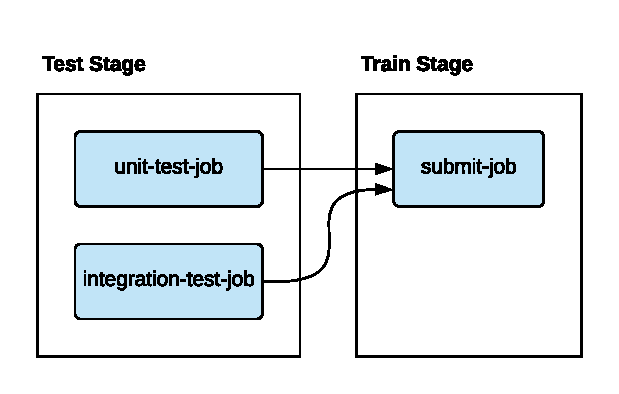
\includegraphics[scale=1]{images/05_conceptual_design/automated_deployment_pipeline/ci_cd_concept}
\caption{Automated Deployment Pipeline concept}
\label{fig:05_deployment_concept}
\end{figure}
% Short intro
\Fig{fig:05_deployment_concept} illustrates the conceptual design of the \hyperlink{abbr:ci}{CI} pipeline, which consists of two stages:
\begin{enumerate}
\item Test stage: Responsible for performing all tests to validate the application source code.
\item Train stage: If the test stage is successful, the application is submitted to the Apache Spark cluster, in order to train the model.
\end{enumerate}
% No build stage
It is important to mention that a build stage is missing in this conceptual design. The build stage includes compiling source code into a format that can be executed directly.
% Python
Python is an interpreted language and does not need to be compiled for execution.


\subsection{Test Stage}
% short intro
Before training the machine learning model, the application source must be validated by a series of tests, which can include:
% Tests
\begin{itemize}
\item Unit tests
\item Integration tests
\item End-to-end tests
\end{itemize}
% Different jobs
Each test is performed as a separate job. All jobs perform in parallel after the test stage has been triggered.
% On failure
If a job fails, the whole test stage is marked as a failure, which notifies participating developers.


\subsection{Train Stage}
\paragraph{}
% Short intro
The train stage is responsible for submitting the Apache Spark application to the Apache cluster after the test stage was successful.
% How
A \textit{spark-submit} Docker container has to be deployed to the same Docker network to submit an application to the Apache Spark cluster. How a \textit{spark-submit} container performs an application, is explained in \Sec{subsec:05_spark_spark-submit}.

\paragraph{}
% Same machine with runner
Deploying \textit{spark-submit} Docker containers in the Apache Spark cluster network requires access to the overlying Docker engine.
To access the Docker engine within a job of the train stage, the job has to be executed by a GitLab runner on the same host machine.
% Perform train stage concept
\begin{figure}[h]
\centering
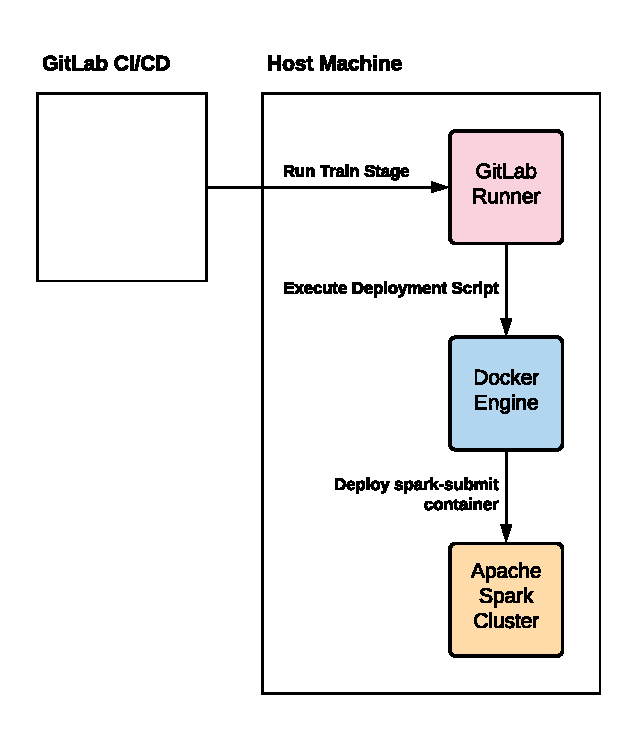
\includegraphics[scale=1]{images/05_conceptual_design/automated_deployment_pipeline/train_stage_runner}
\caption{Deployment of a spark-submit container}
\label{fig:05_deployment_train_concept}
\end{figure}
% Explain figure
\Fig{fig:05_deployment_train_concept} illustrates the steps to deploy a \textit{spark-submit} container in the Apache Spark cluster swarm network.
% Runner
The GitLab CI/CD server connects to a GitLab instance on the host machine and instructs it to execute the train stage.
The runner then performs the scripts that instruct the Docker engine to deploy a spark-submit container in the Apache Spark cluster.
